
\documentclass{beamer}
\usetheme{Electromagnetism}
\usepackage{Electromagnetism}
\graphicspath{{pictures/}}
% -------------------------------------- Grid
%-------------------------------------------------------
\makeatletter
\def\grd@save@target#1{%
  \def\grd@target{#1}}
\def\grd@save@start#1{%
  \def\grd@start{#1}}
\tikzset{
  grid with coordinates/.style={
    to path={%
      \pgfextra{%
        \edef\grd@@target{(\tikztotarget)}%
        \tikz@scan@one@point\grd@save@target\grd@@target\relax
        \edef\grd@@start{(\tikztostart)}%
        \tikz@scan@one@point\grd@save@start\grd@@start\relax
        \draw[minor help lines] (\tikztostart) grid (\tikztotarget);
        \draw[major help lines] (\tikztostart) grid (\tikztotarget);
        \grd@start
        \pgfmathsetmacro{\grd@xa}{\the\pgf@x/1cm}
        \pgfmathsetmacro{\grd@ya}{\the\pgf@y/1cm}
        \grd@target
        \pgfmathsetmacro{\grd@xb}{\the\pgf@x/1cm}
        \pgfmathsetmacro{\grd@yb}{\the\pgf@y/1cm}
        \pgfmathsetmacro{\grd@xc}{\grd@xa + \pgfkeysvalueof{/tikz/grid with coordinates/major step}}
        \pgfmathsetmacro{\grd@yc}{\grd@ya + \pgfkeysvalueof{/tikz/grid with coordinates/major step}}
        \foreach \x in {\grd@xa,\grd@xc,...,\grd@xb}
        \node[anchor=north] at (\x,\grd@ya) {\pgfmathprintnumber{\x}};
        \foreach \y in {\grd@ya,\grd@yc,...,\grd@yb}
        \node[anchor=east] at (\grd@xa,\y) {\pgfmathprintnumber{\y}};
      }
    }
  },
  minor help lines/.style={
    help lines,
    step=\pgfkeysvalueof{/tikz/grid with coordinates/minor step}
  },
  major help lines/.style={
    help lines,
    line width= 0.5pt,
    step=\pgfkeysvalueof{/tikz/grid with coordinates/major step}
  },
  grid with coordinates/.cd,
  minor step/.initial=.2,
  major step/.initial=1,
  major line width/.initial=2pt,
}
\makeatother
\usepackage{cancel}
\begin{document}


% ============================== Слайд ## ===================================
\begin{frame}[fragile]{Густини електричного заряду}{}

\begin{center}
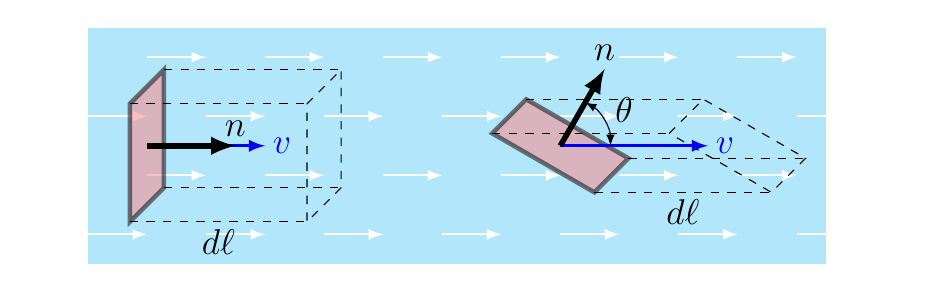
\begin{tikzpicture}[>=latex, scale=0.75, transform shape, every node/.style={font=\LARGE}]
%\clip (-0.5,0.5) rectangle (14.5, -3.5);
\fill[cyan, opacity=0.3] (1,0.5) rectangle (13.5, -3.5);
\foreach \x in {0,...,7} {
    \foreach \y in {0,-2} {
        \draw[->, thick, white] ({2*\x}, \y) -- ++(1, 0);
        \ifnum\x<7
            \ifnum\y>-4
            \draw[->, thick, white] ({2*\x + 1}, {\y-1}) -- ++(1, 0);
            \fi
        \fi
    }
}


\tikzset{
surface/.pic ={
    \def\h{2}
    \def\w{1.5}
    \path[pic actions] (0, \h, \w) coordinate (-A)
    -- (0,  \h, -\w) coordinate (-B)
    -- (0, -\h, -\w) coordinate (-C)
    -- (0, -\h,  \w) coordinate (-D)
    --cycle;
    \coordinate (-c) at (0, 0, 0);
    }
}


\begin{scope}[scale=1, yshift=-1.5cm,]
    \pic[scale=0.5, fill=red!50, opacity=0.5, draw, ultra thick] (S) at (2, 0) {surface};
    \draw[->, blue, line width=1pt] (S-c) -- ++(2,0) node[right] {$\vect{v}$};
    \draw[->, line width=2pt] (S-c) -- ++(1.5,0) node[above] {$\vect{n}$};
    \draw[dashed] (S-A) -- ++(3,0);
    \draw[dashed] (S-B) -- ++(3,0);
    \draw[dashed] (S-C) -- ++(3,0);
    \draw[dashed] (S-D) -- node[below] {$d\ell$} ++(3,0);
    \pic[scale=0.5, dashed, draw] at (5, 0) {surface};
\end{scope}

\begin{scope}[scale=1, shift={(9, -1.5)}]
    \def\a{60}
    \pic[scale=0.5, fill=red!50, opacity=0.5, draw, ultra thick, rotate around z=\a] (S) at (0, 0) {surface};
    \pic[scale=0.5, draw, dashed, rotate around z=\a, xshift=6cm] at (0,0) {surface};
    \draw[->, blue, line width=1pt] (S-c) -- ++(2.5,0) node[right] {$\vect{v}$};
    \draw[->, line width=2pt] (S-c) -- ++(\a:1.5) node[above] {$\vect{n}$};
    \draw[dashed] (S-A) -- ++(3,0);
    \draw[dashed] (S-B) -- ++(3,0);
    \draw[dashed] (S-C) -- ++(3,0);
    \draw[dashed] (S-D) -- node[below] {$d\ell$} ++(3,0);
    \draw[<->] (0, 0) ++(0:0.85) arc(0:\a:0.85) node[pos=0.3, anchor=south west] {$\theta$};
\end{scope}
\end{tikzpicture}
\end{center}

\end{frame}
% ===========================================================================


\end{document}